\section {Especificaci\'on de requisitos}

\subsection {Interfaces externos}

\textbf{Interfaces de usuario:}\\

La interfaz de uso proporciona todo lo necesario para controlar la aplicación en su totalidad.\\

\textbf{Interfaces de hardware:}\\

Se debe disponer de un dispositivo móvil y un ordenador.\\

\textbf{Interfaces de software:}\\

La versión de Android del dispositivo móvil debe ser la 4.0 o superior.\\

El en la máquina remota se debe disponer de una aplicación VNC de tipo servidor.\\

\textbf{Interfaces de comunicación:}\\

Tanto el cliente como el servidor deben disponer de una conexión a internet o estar ambos en la misma red local.\\

\subsection {Funciones}

Los siguientes requisitos funcionales definen las acciones que deben tener lugar en el software, aceptando y precesando las entradas y procesando y generando las salidas.\\

\textbf{Crear conexión:}
\begin{itemize}
\item Prioridad: Alta.
\item Estabilidad: Alta.
\item Descripción: Crea una nueva conexión y la añade a la lista de conexiones.
\item Entrada: Nombre de la conexión, IP, puerto, contraseña y calidad de imagen.
\item Salida: La conexión se añade a la lista.
\item Origen: Usuario.
\item Destino: Aplicación.
\item Necesita:
\item Acción: Crea una nueva conexión.
\item Precondición:
\item Postcondición: La conexión se añade a la lista de conexiones.
\item Efectos laterales: N/A.\\

\end{itemize}

\textbf{Editar conexión:}
\begin{itemize}
\item Prioridad: Alta.
\item Estabilidad: Alta.
\item Descripción: Se editan los datos de una determinada conexión.
\item Entrada: Nombre de la conexión, IP, puerto, contraseña y calidad de imagen.
\item Salida: La conexión con los datos modificados.
\item Origen: Usuario.
\item Destino: Aplicación.
\item Necesita:
\item Acción: Edita los datos de una conexión.
\item Precondición:
\item Postcondición: Los datos de la conexión se modifican.
\item Efectos laterales: N/A.\\

\end{itemize}

\textbf{Borrar conexión:}
\begin{itemize}
\item Prioridad: Alta.
\item Estabilidad: Alta.
\item Descripción: Se elimina una conexión.
\item Entrada:
\item Salida: La conexión se elimina de la aplicación.
\item Origen: Usuario.
\item Destino: Aplicación.
\item Necesita:
\item Acción: Elimina una conexión.
\item Precondición:
\item Postcondición: La conexión se borra de la aplicación.
\item Efectos laterales: Si la conexión esta en favoritos se borrará también ahí.\\

\end{itemize}

\textbf{Ver información de la conexión:}
\begin{itemize}
\item Prioridad: Alta.
\item Estabilidad: Alta.
\item Descripción: Muestra la información de una conexión.
\item Entrada:
\item Salida: Los datos de la conexión.
\item Origen: Usuario.
\item Destino: Usuario.
\item Necesita:
\item Acción: Muestra los datos de una conexión.
\item Precondición:
\item Postcondición: Se muestran los datos de una conexión.
\item Efectos laterales: N/A.\\

\end{itemize}

\textbf{Añadir conexión a favoritos:}
\begin{itemize}
\item Prioridad: Alta.
\item Estabilidad: Alta.
\item Descripción: Añade una conexión a la lista de favoritos del usuario.
\item Entrada: La conexión.
\item Salida: La conexión se añade a la lista de favoritos.
\item Origen: Usuario.
\item Destino: Aplicación.
\item Necesita: Acceso a la base de datos.
\item Acción: Añade la conexión a la lista de favoritos.
\item Precondición:
\item Postcondición: La conexión se añade a favoritos.
\item Efectos laterales: N/A.\\

\end{itemize}

\textbf{Borrar conexión de favoritos:}
\begin{itemize}
\item Prioridad: Alta.
\item Estabilidad: Alta.
\item Descripción: Borra una conexión de la lista de favoritos.
\item Entrada:
\item Salida: La conexión se elimina de favoritos.
\item Origen: Usuario.
\item Destino: Aplicación.
\item Necesita: Acceso a la base de datos.
\item Acción: Elimina una conexión de la lista de favoritos.
\item Precondición:
\item Postcondición: La conexión se borra de favoritos.
\item Efectos laterales: N/A.\\

\end{itemize}

\textbf{Ver lista de conexiones:}
\begin{itemize}
\item Prioridad: Alta.
\item Estabilidad: Alta.
\item Descripción: Se muestran todas las conexiones recientes.
\item Entrada:
\item Salida: La lista de conexiones recientes.
\item Origen: Usuario.
\item Destino: Usuario.
\item Necesita:
\item Acción: Se muestran las conexiones recientes.
\item Precondición: Tiene que existir al menos una conexión reciente.
\item Postcondición: Se muestra la lista de conexiones recientes.
\item Efectos laterales: N/A.\\

\end{itemize}

\textbf{Ver lista de conexiones favoritas:}
\begin{itemize}
\item Prioridad: Alta.
\item Estabilidad: Alta.
\item Descripción: Se muestran todas las conexiones favoritas.
\item Entrada:
\item Salida: La lista de conexiones favoritas.
\item Origen: Usuario.
\item Destino: Usuario.
\item Necesita:
\item Acción: Se muestran las conexiones favoritas.
\item Precondición: Tiene que existir al menos una conexión favorita.
\item Postcondición: Se muestra la lista de conexiones favoritas.
\item Efectos laterales: N/A.\\

\end{itemize}

\textbf{Abrir menú principal:}
\begin{itemize}
\item Prioridad: Alta.
\item Estabilidad: Alta.
\item Descripción: Se abre el menú principal.
\item Entrada:
\item Salida: Se muestra el menú.
\item Origen: Usuario.
\item Destino: Usuario.
\item Necesita:
\item Acción: Se muestra el menú principal.
\item Precondición:
\item Postcondición: Se muestra el menú principal.
\item Efectos laterales: N/A.\\

\end{itemize}

\textbf{Conectarse:}

\begin{itemize}
\item Prioridad: Alta.
\item Estabilidad: Alta.
\item Descripción: Se conecta al servidor especificado en los datos de la conexión.
\item Entrada: Datos de la conexión.
\item Salida: Conexión con el servidor.
\item Origen: Usuario.
\item Destino: Usuario.
\item Necesita:
\item Acción: Se conecta con el servidor remoto.
\item Precondición: El servidor tiene que tener ejecutandose una aplicación VNC.
\item Postcondición: El cliente se conecta con el servidor.
\item Efectos laterales: N/A.\\

\end{itemize}

\textbf{Desconectarse:}
\begin{itemize}
\item Prioridad: Alta.
\item Estabilidad: Alta.
\item Descripción: Se desconecta del servidor al que se estaba conectado.
\item Entrada:
\item Salida: Desconexión con el servidor.
\item Origen: Usuario.
\item Destino: Usuario.
\item Necesita: Estar conectado.
\item Acción: Se desconecta del servidor remoto.
\item Precondición: Se debe estar conectado para poder desconectarse.
\item Postcondición: El cliente se desconecta del servidor.
\item Efectos laterales: N/A.\\

\end{itemize}

\textbf{Hacer click:}
\begin{itemize}
\item Prioridad: Alta.
\item Estabilidad: Alta.
\item Descripción: Se envía la orden de pulsar el botón izquierdo del ratón.
\item Entrada:
\item Salida:
\item Origen: Usuario.
\item Destino: Aplicación.
\item Necesita: Estar conectado.
\item Acción: Se envía la orden de hacer click.
\item Precondición: Se debe estar conectado.
\item Postcondición: Se envía la orden de hacer click.
\item Efectos laterales: N/A.\\

\end{itemize}

\textbf{Pulsar botón derecho:}
\begin{itemize}
\item Prioridad: Alta.
\item Estabilidad: Alta.
\item Descripción: Se envía la orden de pulsar el botón derecho del ratón.
\item Entrada:
\item Salida:
\item Origen: Usuario.
\item Destino: Aplicación.
\item Necesita: Estar conectado.
\item Acción: Se envía la orden de hacer click en el botón derecho.
\item Precondición: Se debe estar conectado.
\item Postcondición: Se envía la orden de hacer click en el botón derecho.
\item Efectos laterales: N/A.\\

\end{itemize}

\textbf{Moverse por el escritorio:}
\begin{itemize}
\item Prioridad: Alta.
\item Estabilidad: Alta.
\item Descripción: Movimientos por la imagen del escritorio del servidor.
\item Entrada:
\item Salida:
\item Origen: Usuario.
\item Destino: Usuario.
\item Necesita: Estar conectado.
\item Acción: Se muestran diferentes partes del escritorio según el movimiento.
\item Precondición: Se debe estar conectado.
\item Postcondición: Se muestra una nueva imagen del escritorio.
\item Efectos laterales: N/A.\\

\end{itemize}

\textbf{Abrir menú de conexión:}
\begin{itemize}
\item Prioridad: Alta.
\item Estabilidad: Alta.
\item Descripción: Se abre el menú de opciones.
\item Entrada:
\item Salida: Se muestra el menú.
\item Origen: Usuario.
\item Destino: Usuario.
\item Necesita: Estar conectado.
\item Acción: Se muestra el menú de conexión.
\item Precondición: Se debe estar conectado.
\item Postcondición: Se muestra el menú de conexión.
\item Efectos laterales: N/A.\\

\end{itemize}

\textbf{Abrir teclado:}
\begin{itemize}
\item Prioridad: Alta.
\item Estabilidad: Alta.
\item Descripción: Se muestra el teclado para poder enviar teclas.
\item Entrada:
\item Salida: Se muestra el teclado en pantalla.
\item Origen: Usuario.
\item Destino: Usuario.
\item Necesita: Estar conectado.
\item Acción: Se muestra el teclado.
\item Precondición: Se debe estar conectado.
\item Postcondición: Se muestra el teclado en pantalla.
\item Efectos laterales: N/A.\\

\end{itemize}

\textbf{Enviar pulsaciones de teclas:}
\begin{itemize}
\item Prioridad: Alta.
\item Estabilidad: Alta.
\item Descripción: Se envían pulsaciones de teclas.
\item Entrada: Una pulsación de tecla.
\item Salida:
\item Origen: Usuario.
\item Destino: Aplicación.
\item Necesita: Estar conectado.
\item Acción: Se envía la orden de pulsar una determinada tecla.
\item Precondición: Se debe estar conectado.
\item Postcondición: Se envía la orden de pulsar una tecla.
\item Efectos laterales: N/A.\\

\end{itemize}

\textbf{Enviar combinaciones de teclas:}
\begin{itemize}
\item Prioridad: Alta.
\item Estabilidad: Alta.
\item Descripción: Se envían combinaciones de teclas.
\item Entrada: Una pulsación de una combinación de teclas.
\item Salida:
\item Origen: Usuario.
\item Destino: Aplicación.
\item Necesita: Estar conectado.
\item Acción: Se envía la orden de pulsar una combinación de teclas.
\item Precondición: Se debe estar conectado.
\item Postcondición: Se envía la orden de pulsar una combinación de teclas.
\item Efectos laterales: N/A.\\

\end{itemize}

\textbf{Centrar la imagen:}
\begin{itemize}
\item Prioridad: Alta.
\item Estabilidad: Alta.
\item Descripción: Se centra la imagen en la esquina superior izquierda del escritorio remoto.
\item Entrada:
\item Salida:
\item Origen: Usuario.
\item Destino: Usuario.
\item Necesita: Estar conectado.
\item Acción: Se centra la imagen.
\item Precondición: Se debe estar conectado.
\item Postcondición: Se centra la imagen en la esquina superior izquierda.
\item Efectos laterales: N/A.\\

\end{itemize}

\textbf{Hacer zoom en la imagen:}
\begin{itemize}
\item Prioridad: Alta.
\item Estabilidad: Alta.
\item Descripción: Se hace zoom en una determinada zona del escritorio.
\item Entrada:
\item Salida:
\item Origen: Usuario.
\item Destino: Usuario.
\item Necesita: Estar conectado.
\item Acción: Se hace zoom en la imagen del escritorio.
\item Precondición: Se debe estar conectado.
\item Postcondición: Se hace zoom.
\item Efectos laterales: N/A.\\

\end{itemize}

\section {Diagramas de clases}

\begin{figure}[h] %[h] para here [b] para bottom [t] para top
\begin{center}
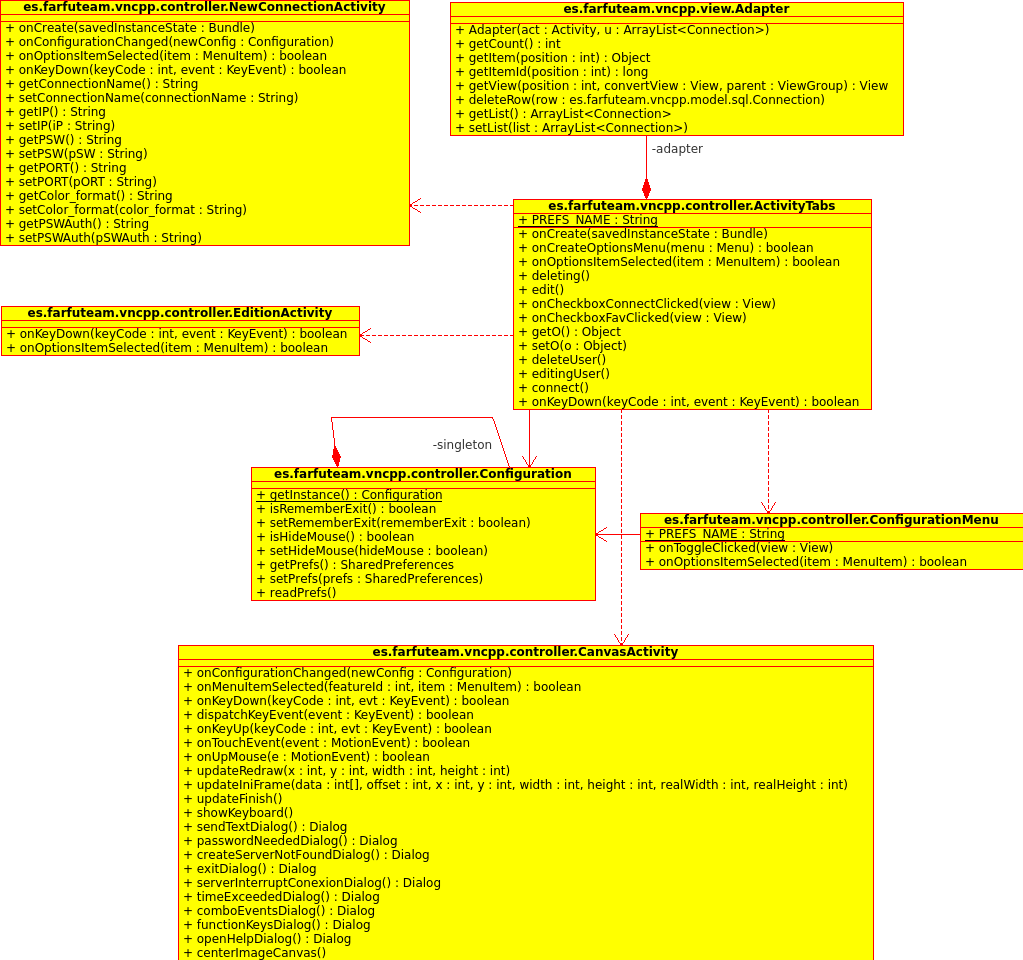
\includegraphics[height= 11 cm , width=16 cm]{Main.png}
\end{center}
\caption{Diagrama principal}
\end{figure}
